\subsubsection{Minuta de reunião (10-Dezembro-2015)}

\begin{tabbing}
  Local \= xxx \kill
  Local \> : LEAD \\
  Data  \> : 10 de Dezembro de 2015 \\
  Hora  \> : 10:00
\end{tabbing} 

%---------------------------------------------------------------------
\participantes{
  \gabriel,
  \julia,
  \estevão,
  \elael,
  \renan,
  \ramon.

}

\textbf{Aprovação da minuta}

\textbf{Update semanal do Projeto EMMA}
   									
						
\textbf{\gabriel.} 
	\begin{itemize}
			\item Compra do Sensor a laser da empesa Faro enviada.
			\end{itemize}
		
		\item \textbf{Novas tarefas:}
			\begin{itemize} 
				\item Trabalho em andamento do com Point Cloud e PCL.
				\item Pesquisou possibilidade para 'oclusão'.
			\end{itemize}

					
   \textbf{\estevão.} 
	\begin{itemize}
		\item \textbf{Tarefas concluídas:}
			\begin{itemize}    
			    \item Definiu aspectos técnicos para a cotação do braço mecânico
			    Motoman MH12.
			    \item Coloborou com Renan para estudos de simulações.
				
			\end{itemize}
		
		\item \textbf{Novas tarefas:}
			\begin{itemize} 
			    \item Ajustes no desenho da base.
			\end{itemize}
	\end{itemize}

	
	  \textbf{\elael.} 
	\begin{itemize}
		\item \textbf{Tarefas concluídas:}
			\begin{itemize}    
				\item Pesquisa bibliográfica para o segundo artigo do
				EMMA-DETAIL: Estudo do conceito para metodologia e revestimento robótico
de turbinas.
			\end{itemize}
		
		\item \textbf{Novas tarefas:}
			\begin{itemize} 
			    \item Dar início ao segundo artigo do EMMA-DETAIL, Estudo do conceito para metodologia e revestimento robótico
de turbinas.
			\end{itemize}
	\end{itemize}			
			
  \textbf{\renan.} 
	\begin{itemize}
		\item \textbf{Tarefas concluídas:}
			\begin{itemize}    
				\item Executou diferentes simulações nos softwares MoveIt e no OpenRave.
			\end{itemize}
		
		\item \textbf{Novas tarefas:}
			\begin{itemize} 
			    \item Formalizar simulações em um relatório.
			\end{itemize}
	\end{itemize}	
			
   \textbf{\julia.} 
	\begin{itemize}
		\item \textbf{Tarefas concluídas:}
			\begin{itemize}    
				\item Descrição de tarefas: calibração, planejamento de trajetória e metalização para artigo.
				\item Cobrar testes do grupo formado para questionários da pesquisa.
			\end{itemize}
		
		\item \textbf{Novas tarefas:}
			\begin{itemize} 
			    \item Formato de artigo para interface de usuário EMMA.
			\end{itemize}
	\end{itemize}		



\textbf{Agenda para a próxima reunião:}
  \begin{itemize}
    \item Resultado de pesquisas individuais.
    \item Novas tarefas \& recomendações.
  \end{itemize}


\vspace{5mm}%
\parbox[t]{70mm}{
  Aprovado por: \\[5mm]
  \centering
  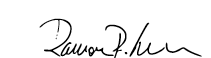
\includegraphics[width=65mm]{figs/logo/assinatura-ramon.png} \\[-4mm]
  \rule[2mm]{70mm}{0.1mm} \\
  \ramon \\[1mm]
  Coordenador do Projeto \\
}

%---------------------------------------------------------------------
\fim